\section{Preliminary Evaluation}
\label{sec:eval}

% \begin{itemize}
%   \item Experiment on datas from the Bureau of Transportation Statistic (\url{http://www.transtats.bts.gov/Fields.asp?Table_ID=236}) to evaluate flight delays by airport
%   \item Infrastructure based on ONE cluster, VM 16.04 LTS (GNU/Linux 4.4.0-53-generic x86\_64), Docker 1.13.0-rc3, Docker Swarm 1.2.5 (discovery: Consul v0.5.2)
%   \item Hardware?
% \end{itemize}

Our preliminary evaluation of \SYS is based on the processing of datas from the Bureau of Transportation Statistic\cite{rita:bts}.
Its goal is to determine average delays and the total of delayed flights for each air carrier.
These datas report flights departures and arrivals\cite{rita:bts} and are available on the website Statiscal Computing\cite{statistical_computing:data}.
They are processed accross a pipeline where they are (i) parsed from CSV to data structure (map), (ii) filtered by relevancy (if the data concerns a delayed flight), and (iii) reduced to compute the wanted insights.
The experiment is done on the 4 last years of the available datas (from 2005 to 2008 included), that being approximatively 28 millions of entries to process.

Scalability of \SYS is evaluated by processing these datas 20 times on 3 different pipeline topology: using 1, 2 or 4 workers for each step of the pipeline.
Results are represented on figure \ref{fig:scalability}, and show clearly better performances between the experiment using only one worker by task, and the one using 2 workers.
In an other hand, using 4 workers instead of 2 does not show any performance improvement.

\begin{figure}[t!]
  \centering
  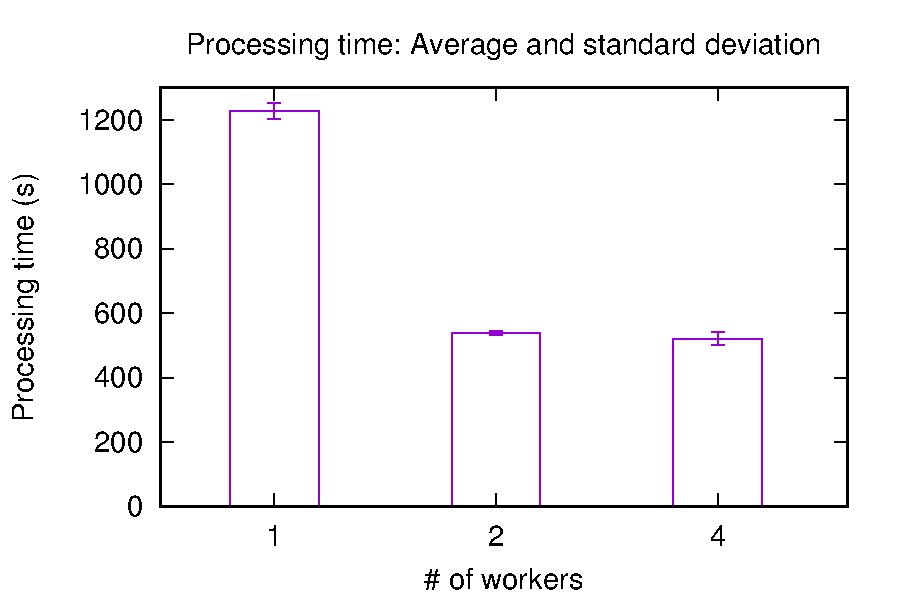
\includegraphics[width=.99\linewidth]{images/avg_stdev_4_streams}
  \caption{Scalability.}
  \label{fig:scalability}
\end{figure}

The latter observation can be explained by the fact that each job in our experiment is very simple and executed too quickly by the workers, compared to the throughput capacity of the communication between two steps of the process pipeline.
This may be due to the limitation of the network bandwith capacity, when the cost of data communication accross nodes is higher than the one of data computation, as described by the Gunther's Universal Law of Computational Scalability\cite{gunther1993simple}, where the relative capacity of a computational platform is inversely proportional to the sum of the levels of contention (e.g., queueing for shared resources) and coherency delay (i.e., latency for data to become consistent) in the system.
In an other hand, it may also be due to the limitation of the router bandwith, the improvement of which is a part of our future work.

\ah{expose throughput results}

\begin{figure}[t!]
  \centering
  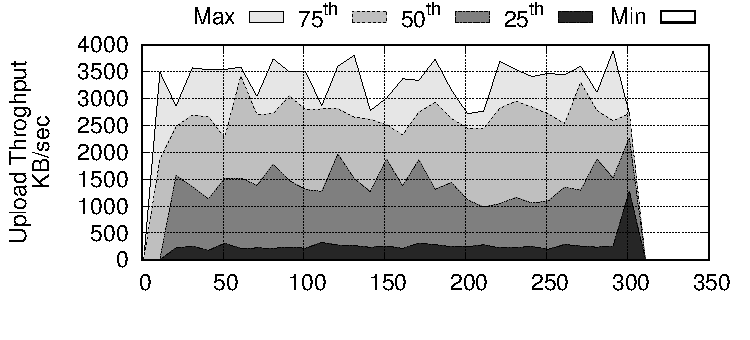
\includegraphics[width=.99\linewidth]{images/tput_upload}
  \caption{Throughput.}
  \label{fig:throughput}
\end{figure}
